\documentclass{article}

% Pass options before loading neurips_2026
\PassOptionsToPackage{numbers,compress}{natbib}
\PassOptionsToPackage{hypertexnames=false}{hyperref}

% arXiv preprint mode of the NeurIPS 2026 E&D template (from lucky-fold-paper)
\usepackage[eandd,preprint]{neurips_2026}

\usepackage[utf8]{inputenc}
\usepackage[T1]{fontenc}
\usepackage{hyperref}
\usepackage{url}
\usepackage{booktabs}
\usepackage{amsfonts}
\usepackage{amsmath}
\usepackage{amssymb}
\usepackage{nicefrac}
\usepackage{microtype}
\usepackage{xcolor}
\usepackage{graphicx}
\usepackage{tabularx}
\usepackage{float}
\usepackage{enumitem}
\usepackage{placeins}

\setlist[itemize]{itemsep=1pt, topsep=2pt, parsep=0pt, partopsep=0pt}
\setlist[enumerate]{itemsep=1pt, topsep=2pt, parsep=0pt, partopsep=0pt}
\setlength{\abovecaptionskip}{4pt}
\setlength{\belowcaptionskip}{2pt}

\graphicspath{{figures/}{figures/supp/}{tables/}}

% Shorthands for connectome arrows / metric names
\newcommand{\fcsc}{FC$\rightarrow$SC}
\newcommand{\scfc}{SC$\rightarrow$FC}
\newcommand{\dpear}{\texttt{demeaned\_pearson}}
\newcommand{\bvdemo}{\texttt{bv+demo}}

\title{What Cross-Modal Connectome Prediction Does and Does Not Buy}

\author{%
  Adel Sahuc \\
  New York University Tandon School of Engineering \\
  \texttt{ans9868@nyu.edu}%
}

\begin{document}

\maketitle

\begin{abstract}
Cross-modal connectome prediction is often treated as a route from one brain measurement to another: if structural connectivity (SC) can predict functional connectivity (FC), or FC can predict SC, then the predicted connectome may stand in for the missing modality. We tested this assumption in HCP Young Adults using two parcellations, 10 frozen family-aware splits, deterministic estimators, and a grid that separates reconstruction from downstream cognitive utility. Cross-modal prediction was real and directional: FC predicted individual deviations in SC better than SC predicted FC ($1.61\times$ in Glasser and $1.68\times$ in 4S456Parcels with PCA$\rightarrow$PLS). This asymmetry was not explained by within-modality reliability, because FC and SC were similarly self-predictable under oracle same-modality controls. However, reconstruction did not imply downstream utility. A cheap brain-volume plus demographics baseline (\bvdemo) predicted cognition substantially, observed FC provided the only consistent lift over this baseline, observed SC underperformed it, and imputed connectomes did not transfer FC's cognitive signal through SC. In particular, FC imputed from SC was not merely unhelpful but consistently below the \bvdemo{} baseline. Additional sanity checks ruled out several easy explanations: the ceiling was not a PCA artifact, nonlinear models and richer tractography features did not recover the missing signal, scaling trends did not suggest a growing nonlinear gap, and the \scfc{} shortfall was not explained by FC measurement noise. Predicted connectomes did carry family signal, but optimizing reconstruction and optimizing identification selected different information. These results support a reporting standard for connectome translation studies: report individual-deviation reconstruction metrics, always include a cheap subject-information baseline for downstream claims, and separate reconstruction accuracy from utility.
\end{abstract}

\section{Introduction}

Structural and functional connectomes describe the same brain from different measurement perspectives. This has made FC--SC translation an attractive goal: infer the missing modality, compare modalities in a common space, and use the predicted connectome for behavior, cognition, or individual identification. A successful reconstruction number can make this goal look solved.

But connectome translation has two distinct questions. The first is reconstruction: can one modality recover individual deviations in the other? The second is utility: does the recovered connectome carry information that matters for the target analysis? A model can succeed at the first and fail at the second. In neuroimaging, the gap is especially important because many downstream outcomes are already predictable from cheap subject-level information such as age, sex, and anatomy-derived brain volumes.

This paper treats FC--SC prediction as a methods problem rather than a leaderboard problem. We ask what cross-modal prediction proves, what it fails to prove, and which baselines should be required before a predicted connectome is treated as useful. The central checkpoint is a brain-volume plus demographics baseline (\bvdemo). For downstream cognition, beating the group mean is too weak; the connectome must beat subject information that is already available in most imaging studies.

We make four contributions. First, we reproduce and characterize the known \fcsc{} $>$ \scfc{} asymmetry under a deterministic grid across two parcellations and 10 frozen splits. Second, we show that the apparent value of translation changes once cognition is evaluated against \bvdemo: observed FC helps, SC does not, and imputed connectomes do not rescue the gap. Third, we close several escape routes with sanity checks: reduction choice, nonlinear models, richer structural representations, sample-size trends, and FC reliability do not explain away the ceiling in this healthy young adult regime. Fourth, we show that predicted connectomes are not globally useless: they carry family signal, but reconstruction and identification pull on different information.

\section{Data and Evaluation Design}

We used HCP Young Adults subjects with both resting-state FC and diffusion-derived SC available, plus demographics and anatomy-derived brain-volume features. Connectomes were represented as upper-triangle edge vectors. Analyses were run on two parcellations: Glasser (360 regions; 64{,}620 edges) and 4S456Parcels (456 regions; 103{,}740 edges). Splits were frozen once for 10 seeds and reused across reconstruction, downstream prediction, imputation, leak checks, and family analyses. Family-aware splitting kept siblings and twins on the same side of the split.

The primary reconstruction metric was \dpear: the per-subject correlation after subtracting the training-set group mean connectome from both the prediction and target. This is the load-bearing metric because raw Pearson is dominated by the shared population mean structure of the connectome. We also tracked fingerprinting metrics (\texttt{avg\_rank}, \texttt{top1\_acc}) and conventional regression metrics, but these are secondary or diagnostic.

For reconstruction, the main closed-form estimator was PCA(256)$\rightarrow$PLS(64)$\rightarrow$inverse-PCA. We also ran BayesianRidge and KernelRidge controls. For downstream scalar targets, BayesianRidge is the reportable estimator: PCA$\rightarrow$PLS and KernelRidge scalar rows were retained diagnostically but are ill-conditioned and not numerically stable for low-signal scalar regression. Every reported number therefore names its estimator.

The grid separates two axes that are often conflated: the \emph{input set} (FC, SC, brain volumes \texttt{bv}, demographics \texttt{demo}, \bvdemo, observed connectomes plus \bvdemo, and imputed connectomes) and the \emph{estimator} (the mathematical mapping from input to output). For reconstruction, we evaluate \fcsc, \scfc, subject-information baselines, connectome plus subject-information inputs, and same-modality oracle controls. For downstream cognition, we ask whether observed or imputed connectomes improve prediction of CogTotal, CogFluid, and CogCryst over \bvdemo. Sex and age are evaluated as leak checks, not as scientific outcomes.

\begin{figure}[h]
  \centering
  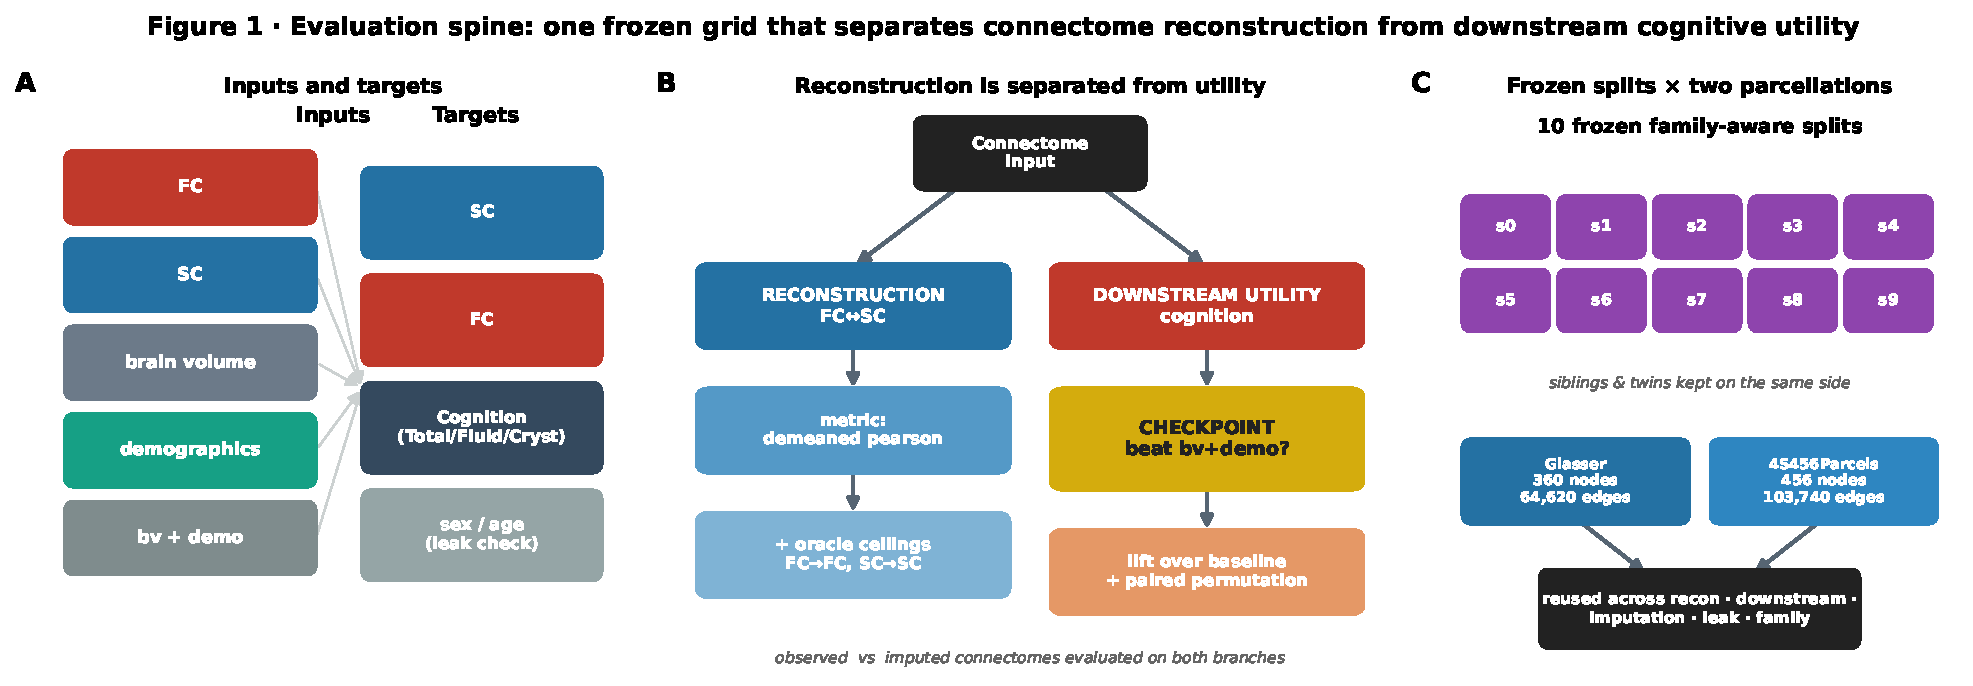
\includegraphics[width=\linewidth]{fig1_evaluation_spine.pdf}
  \caption{\textbf{Evaluation spine.} The study runs one frozen grid that separates connectome reconstruction from downstream cognitive utility, with \bvdemo{} as the checkpoint. (A) inputs and targets; (B) the reconstruction and downstream-utility branches; (C) 10 frozen family-aware splits reused across both parcellations and all analyses.}
  \label{fig:spine}
\end{figure}

\begin{table}[h]
\centering
\caption{Dataset, parcellations, and evaluation.}
\label{tab:dataset}
\small
\begin{tabular}{@{}l p{0.66\linewidth}@{}}
\toprule
\textbf{Field} & \textbf{Value} \\
\midrule
Cohort & HCP Young Adults (FC + SC + demographics + brain-volume) \\
Subjects (per split) & \textasciitilde{}878 (683 train / 195 test, family-aware) \\
Splits & 10 frozen, family-aware (siblings/twins kept on one side) \\
Parcellation A & Glasser --- 360 regions, 64,620 edges \\
Parcellation B & 4S456Parcels --- 456 regions, 103,740 edges \\
Connectome rep. & upper-triangle edge vector \\
Primary recon metric & demeaned\_pearson (per-subject, train-mean removed) \\
Secondary metrics & avg\_rank, top1\_acc (fingerprint), r2/mse \\
Recon estimator & PCA(256)$\rightarrow$PLS(64)$\rightarrow$inverse-PCA (+ BayesianRidge, KernelRidge controls) \\
Downstream estimator & BayesianRidge (reportable for scalar targets) \\
\bottomrule
\end{tabular}
\end{table}

\begin{table}[h]
\centering
\caption{Task grid and the claim each input$\rightarrow$target row tests.}
\label{tab:grid}
\footnotesize
\begin{tabular}{@{}lllllp{0.24\linewidth}@{}}
\toprule
\textbf{Task} & \textbf{Input} & \textbf{Target} & \textbf{Estimator} & \textbf{Metric} & \textbf{Claim tested} \\
\midrule
Reconstruction & FC & SC & PCA$\rightarrow$PLS & demeaned\_pearson & cross-modal FC$\rightarrow$SC \\
Reconstruction & SC & FC & PCA$\rightarrow$PLS & demeaned\_pearson & cross-modal SC$\rightarrow$FC \\
Oracle & FC & FC & BayesianRidge & demeaned\_pearson & within-modality ceiling \\
Oracle & SC & SC & BayesianRidge & demeaned\_pearson & within-modality ceiling \\
Baseline & bv+demo & SC/FC & PCA$\rightarrow$PLS & demeaned\_pearson & subject-info $\rightarrow$ connectome \\
Downstream & bv+demo & Cognition & BayesianRidge & pearson / lift & checkpoint baseline \\
Downstream & obs\_FC & Cognition & BayesianRidge & lift\_over\_bvdemo & does FC beat baseline? \\
Downstream & obs\_SC & Cognition & BayesianRidge & lift\_over\_bvdemo & does SC beat baseline? \\
Downstream & pred\_SC / pred\_FC & Cognition & BayesianRidge & lift\_over\_bvdemo & does imputation transfer? \\
Leak check & any & sex / age & BayesianRidge & bal\_acc / pearson & diagnostic, not outcome \\
Family & pred\_SC variants & MZ/DZ/sib & --- & AUC & identity signal survives? \\
\bottomrule
\end{tabular}
\end{table}

\begin{figure}[h]
  \centering
  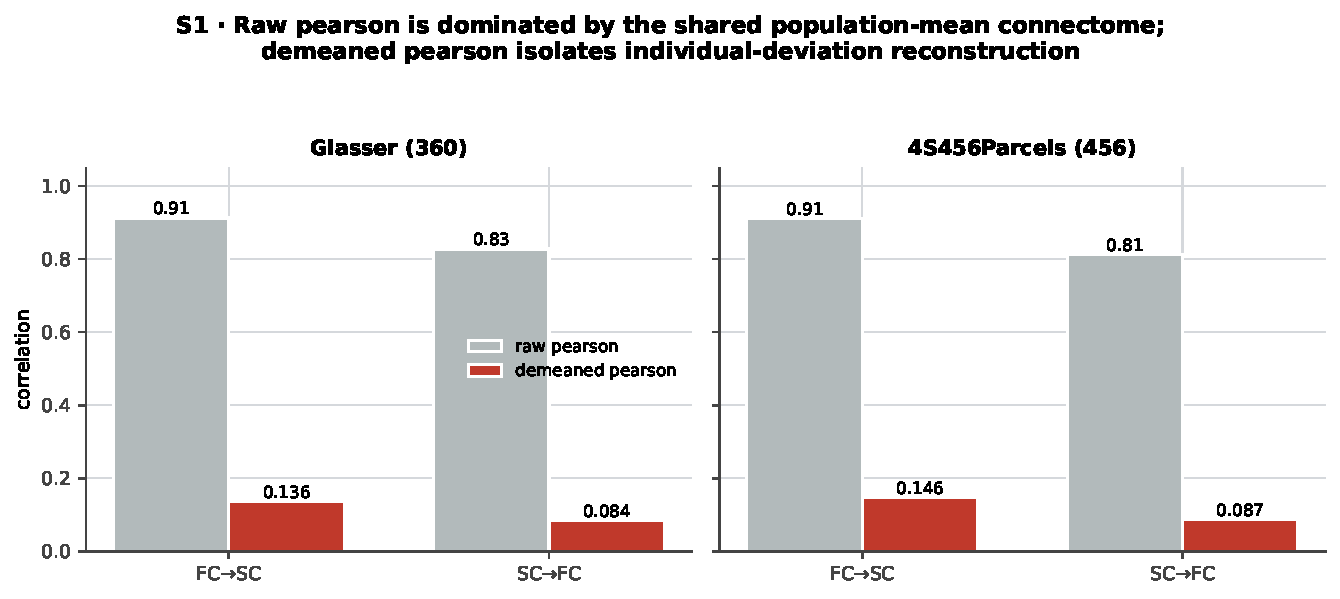
\includegraphics[width=0.82\linewidth]{S1_raw_vs_demeaned.pdf}
  \caption{\textbf{Supplementary: metric choice.} Raw Pearson is dominated by the shared population-mean connectome; \dpear{} isolates individual-deviation reconstruction.}
  \label{fig:s1}
\end{figure}

\begin{figure}[h]
  \centering
  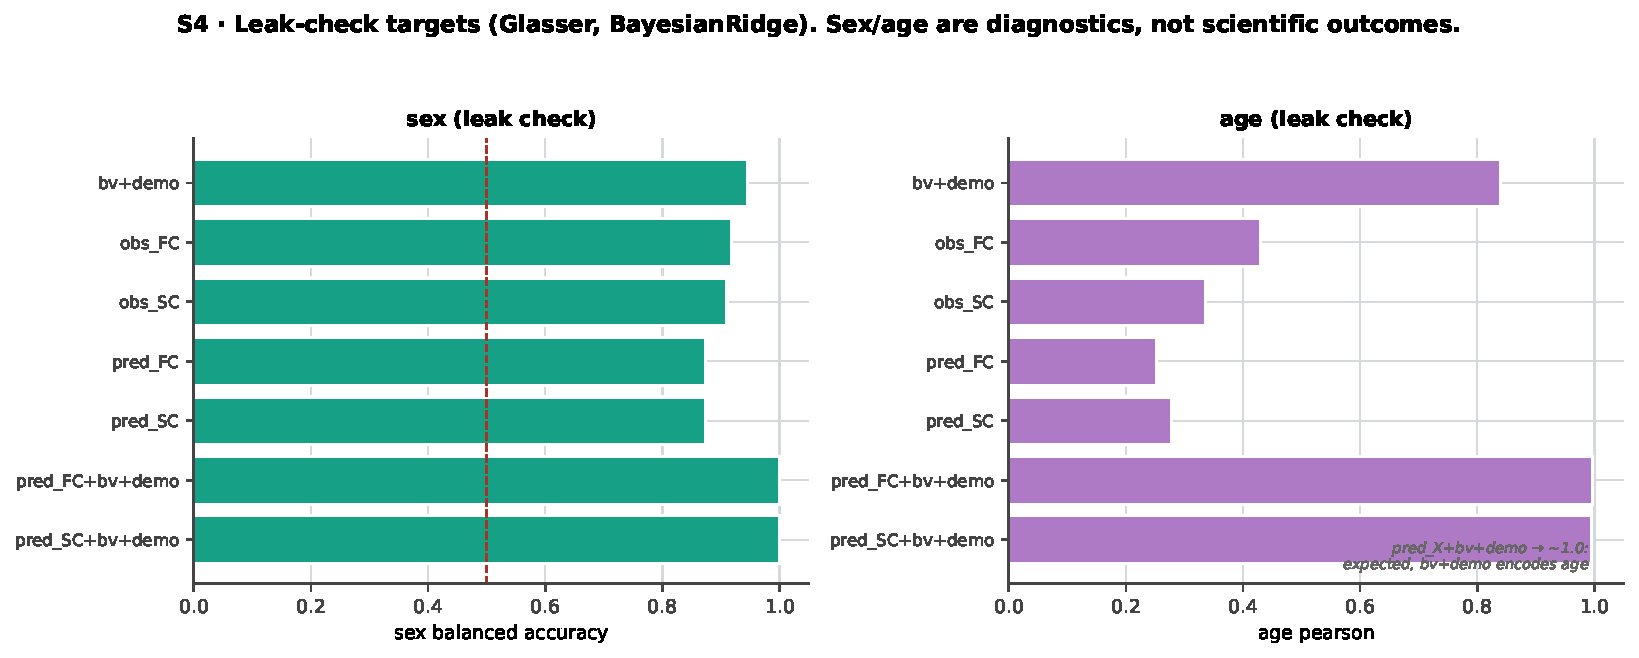
\includegraphics[width=\linewidth]{S4_leak_checks.pdf}
  \caption{\textbf{Supplementary: leak checks.} Sex and age prediction by input (Glasser, BayesianRidge). These are diagnostics, not scientific outcomes.}
  \label{fig:s4}
\end{figure}

\FloatBarrier
\section{Cross-Modal Prediction Is Directional}

FC predicted SC substantially better than SC predicted FC. With PCA$\rightarrow$PLS, the mean \dpear{} across seeds was 0.136 for \fcsc{} and 0.084 for \scfc{} in Glasser, a $1.61\times$ ratio. In 4S456Parcels, \fcsc{} reached 0.146 and \scfc{} 0.087, a $1.68\times$ ratio. The direction was stable across seeds and parcellations (Figure~\ref{fig:directional}).

This asymmetry is not simply because FC or SC is a noisier target. Same-modality oracle controls showed that FC and SC were comparably self-predictable. With BayesianRidge, the \mbox{FC$\rightarrow$FC} oracle was 0.673 in Glasser and 0.632 in 4S456Parcels; the \mbox{SC$\rightarrow$SC} oracle was 0.648 and 0.622 respectively. Thus the target modalities have similar within-modality ceilings, while the cross-modal directions differ strongly.

The baselines also showed a clean double dissociation. Brain-volume features were better predictors of SC than demographics were, whereas demographics were more than twice as predictive of FC as brain volumes were. This crossover matters because it shows that ``subject information'' is not one generic confound. Anatomy and demographics align differently with structure and function.

The finer 4S456Parcels atlas added a useful nuance. Every input$\rightarrow$SC row improved relative to Glasser, while input$\rightarrow$FC rows were slightly lower. The larger parcellation appears to expose more predictable structural detail rather than merely adding noise.

\begin{figure}[h]
  \centering
  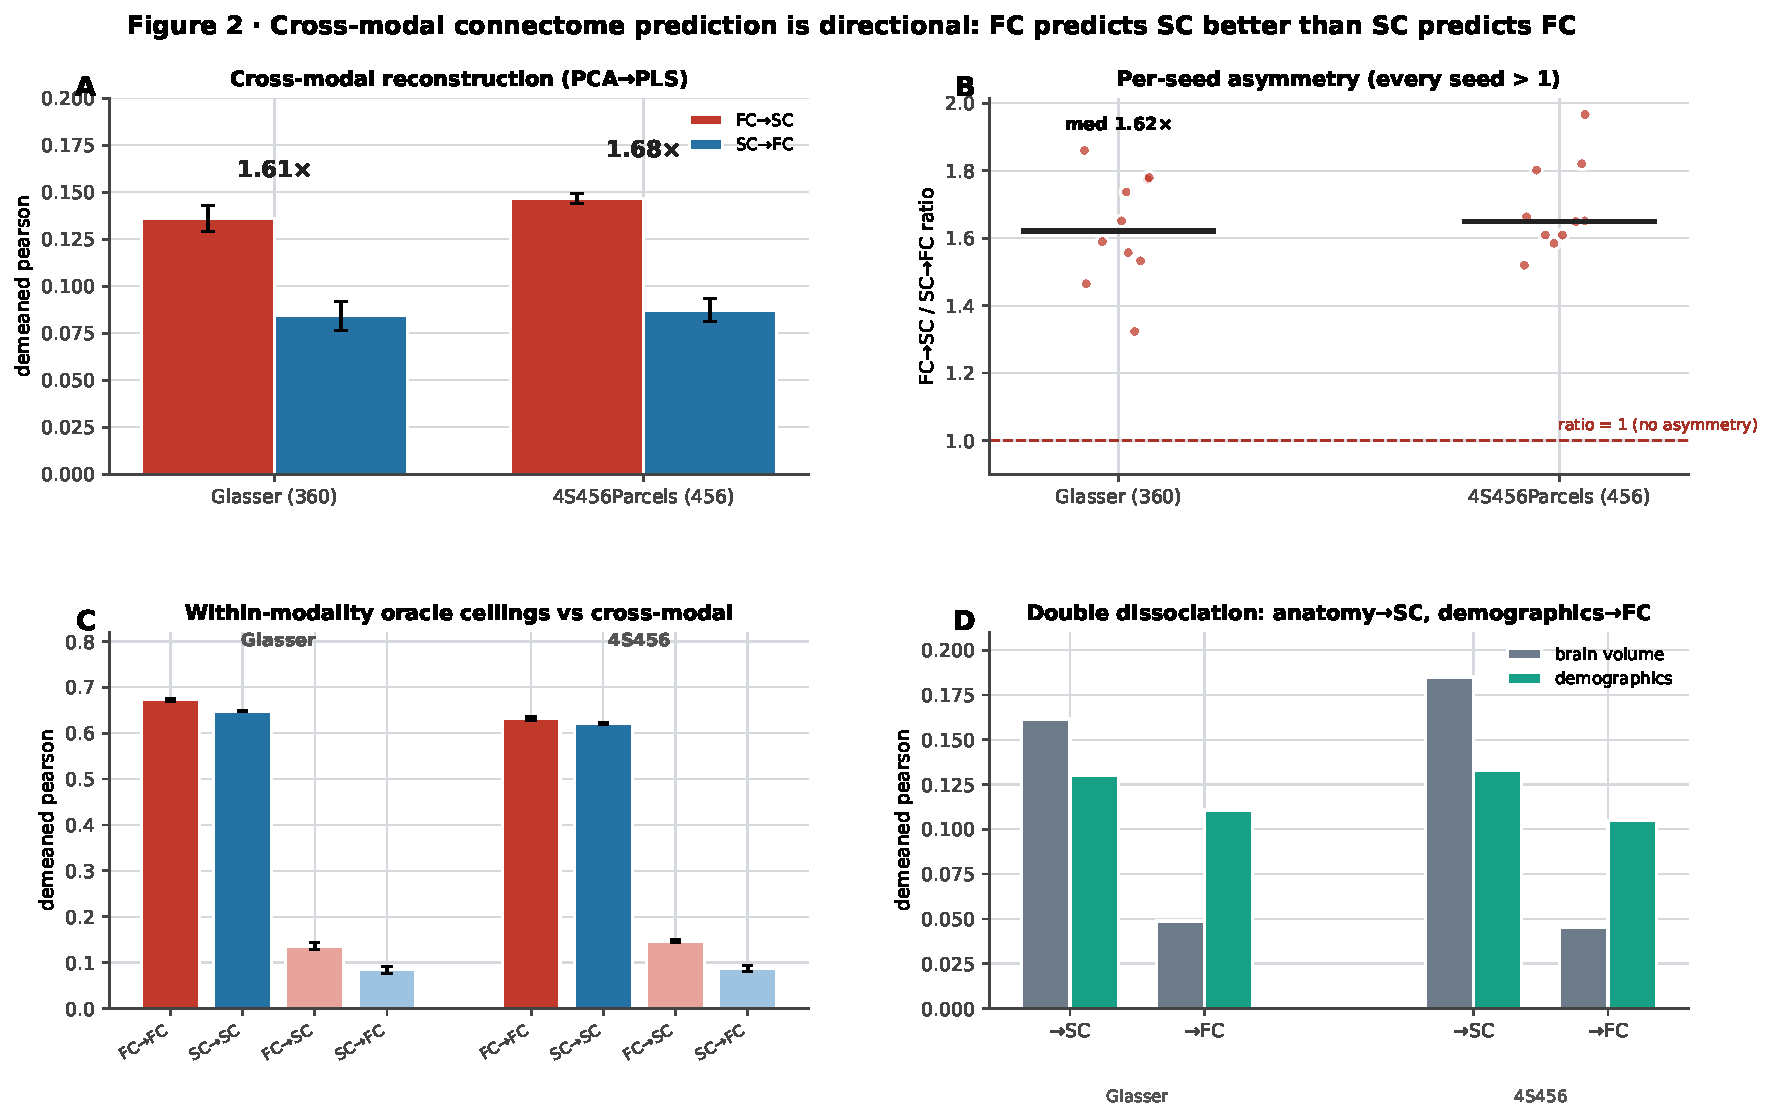
\includegraphics[width=\linewidth]{fig2_directional_translation.pdf}
  \caption{\textbf{Directional translation.} (A) \fcsc{} vs \scfc{} reconstruction (PCA$\rightarrow$PLS); (B) every per-seed ratio exceeds 1; (C) within-modality oracle ceilings are comparable across modalities, far above the cross-modal bars; (D) anatomy predicts SC while demographics predict FC.}
  \label{fig:directional}
\end{figure}

\begin{figure}[h]
  \centering
  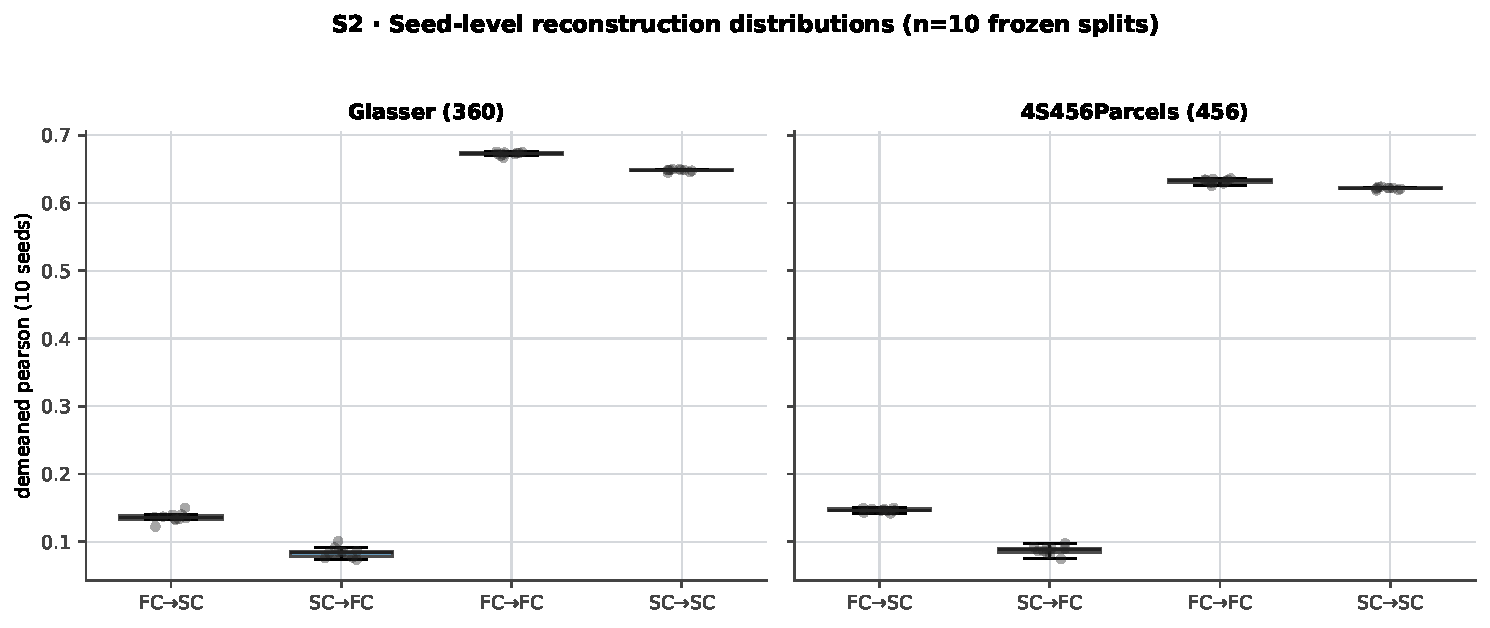
\includegraphics[width=0.88\linewidth]{S2_seed_reconstruction.pdf}
  \caption{\textbf{Supplementary: seed-level reconstruction.} Distributions across the 10 frozen splits for the cross-modal directions and within-modality oracles.}
  \label{fig:s2}
\end{figure}

\FloatBarrier
\section{Reconstruction Does Not Imply Cognitive Utility}

The downstream grid changed the interpretation of cross-modal prediction. The \bvdemo{} baseline itself predicted cognition: with BayesianRidge, CogTotal was 0.359 in both parcellations, CogFluid 0.283, and CogCryst 0.354. This is the bar a connectome must clear.

Observed FC was the only connectome input that consistently improved over this bar. In Glasser, observed FC predicted CogCryst at 0.487, lifting 0.133 over \bvdemo{} with median paired-permutation $p=0.0307$. In 4S456Parcels, observed FC predicted CogCryst at 0.476, lifting 0.122 over baseline with $p=0.0407$. The strongest rows were observed FC plus \bvdemo, especially for CogCryst (0.516 in Glasser, lift 0.162; 0.500 in 4S456Parcels, lift 0.146).

Observed SC did not clear the same baseline. In Glasser, observed SC was below \bvdemo{} for CogTotal, CogFluid, and CogCryst, with lifts of $-0.111$, $-0.120$, and $-0.101$. In 4S456Parcels, the corresponding lifts were $-0.103$, $-0.118$, and $-0.095$.

Imputation did not transfer FC's utility through SC. SC imputed from FC was roughly neutral to slightly below baseline. FC imputed from SC was consistently harmful: in Glasser, \texttt{pred\_FC} lifted CogTotal, CogFluid, and CogCryst by $-0.113$, $-0.097$, and $-0.135$. In 4S456Parcels, the corresponding lifts were $-0.088$, $-0.072$, and $-0.109$. The important point is not merely that imputation failed to help. It injected structured information that made the cognition predictor worse than the cheap subject-information baseline.

These results separate reconstruction from utility. A predicted connectome can be measurable, replicable, and still fail the downstream task it was supposed to enable.

\begin{figure}[h]
  \centering
  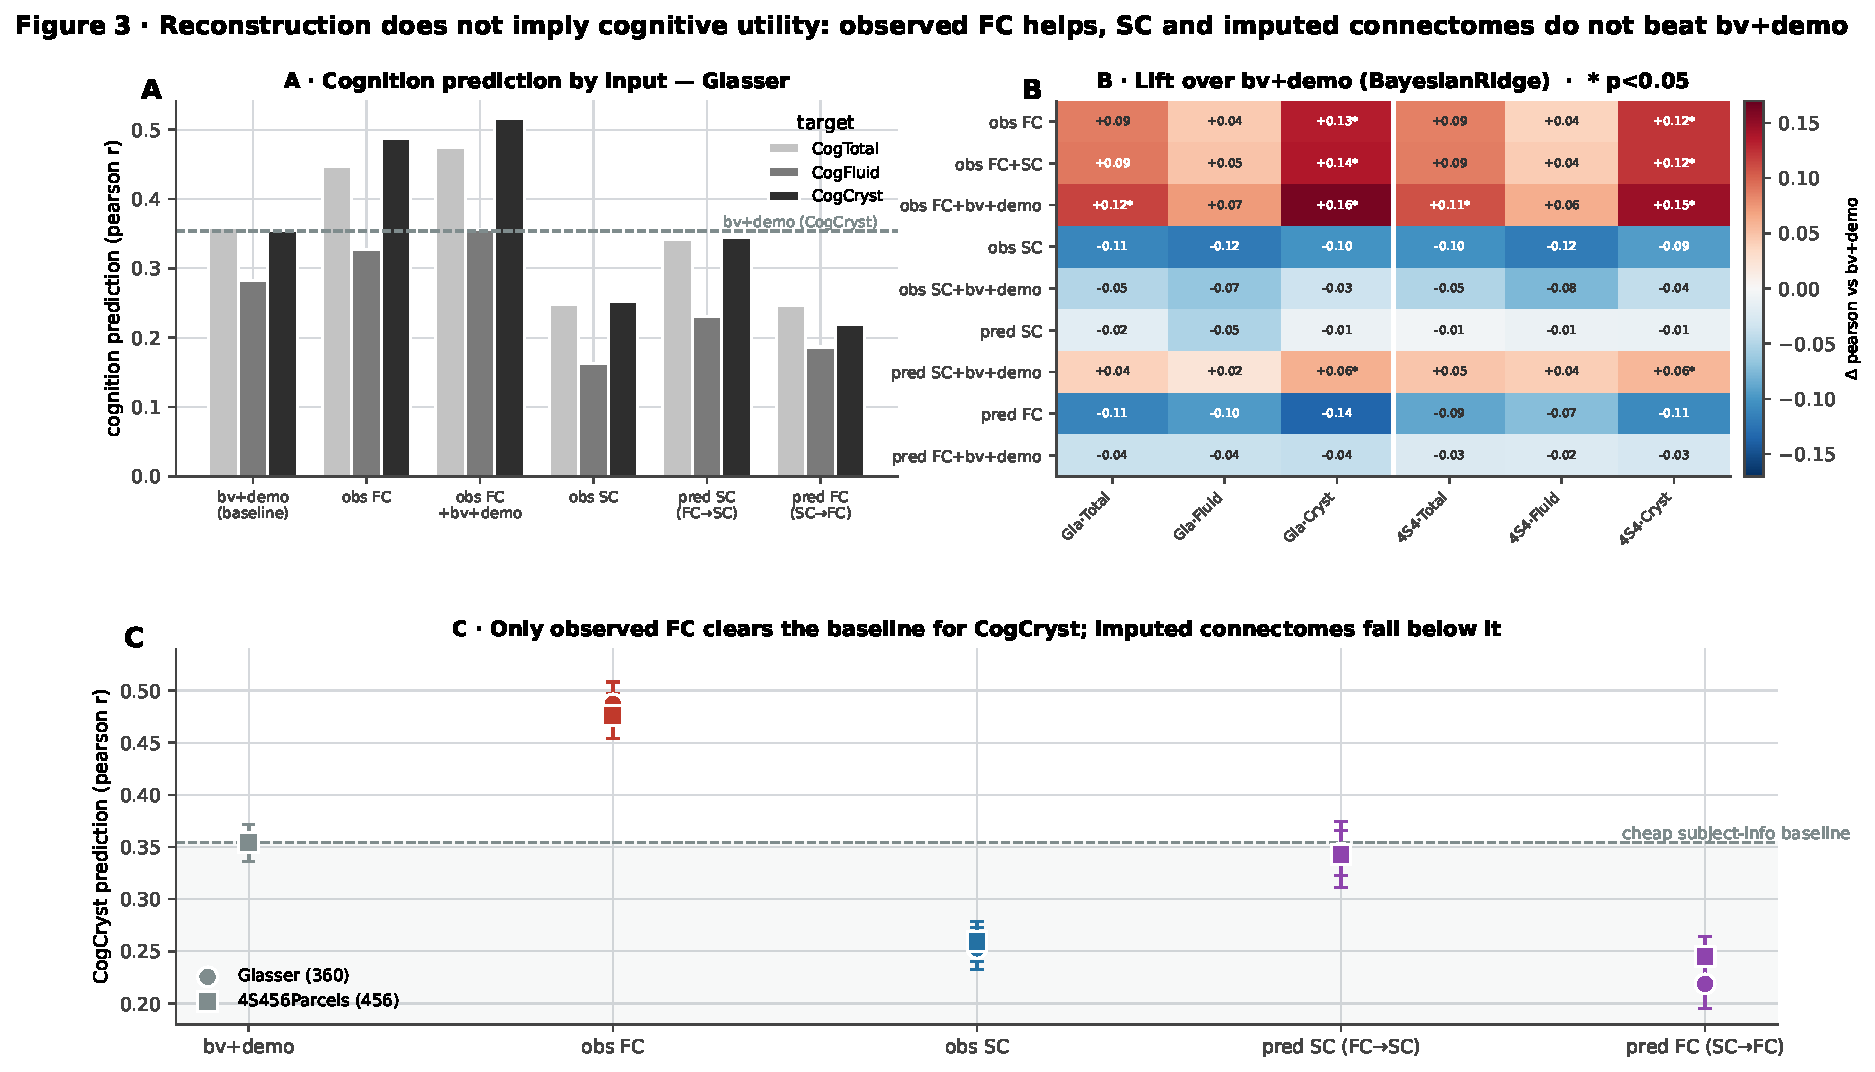
\includegraphics[width=\linewidth]{fig3_utility_checkpoint.pdf}
  \caption{\textbf{Utility checkpoint.} (A) cognition prediction by input (Glasser); (B) lift over \bvdemo{} across both parcellations and three cognitive targets, with paired-permutation significance ($\ast$ $p<0.05$); (C) for CogCryst, only observed FC clears the cheap subject-information baseline, while imputed connectomes fall below it. All downstream numbers are BayesianRidge.}
  \label{fig:utility}
\end{figure}

\begin{table}[h]
\centering
\caption{Headline findings. Values are computed directly from the grid CSVs at build time.}
\label{tab:headline}
\small
\begin{tabular}{@{}lrrlp{0.34\linewidth}@{}}
\toprule
\textbf{Finding} & \textbf{Glasser} & \textbf{4S456} & \textbf{Estimator} & \textbf{Interpretation} \\
\midrule
FC$\rightarrow$SC reconstruction & 0.136 & 0.146 & PCA$\rightarrow$PLS & FC recovers SC deviations \\
SC$\rightarrow$FC reconstruction & 0.084 & 0.087 & PCA$\rightarrow$PLS & weaker reverse direction \\
FC$\rightarrow$SC / SC$\rightarrow$FC ratio & 1.615$\times$ & 1.679$\times$ & PCA$\rightarrow$PLS & directional asymmetry \\
FC$\rightarrow$FC oracle ceiling & 0.673 & 0.632 & BayesianRidge & self-predictability \textasciitilde{}equal \\
SC$\rightarrow$SC oracle ceiling & 0.648 & 0.622 & BayesianRidge & self-predictability \textasciitilde{}equal \\
bv+demo $\rightarrow$ CogCryst & 0.354 & 0.354 & BayesianRidge & the checkpoint to beat \\
obs FC CogCryst lift & +0.133 & +0.122 & BayesianRidge & FC clears the baseline \\
obs SC CogCryst lift & -0.101 & -0.095 & BayesianRidge & SC below baseline \\
pred FC CogCryst lift & -0.135 & -0.109 & BayesianRidge & imputation is harmful \\
\bottomrule
\end{tabular}
\end{table}

\begin{figure}[h]
  \centering
  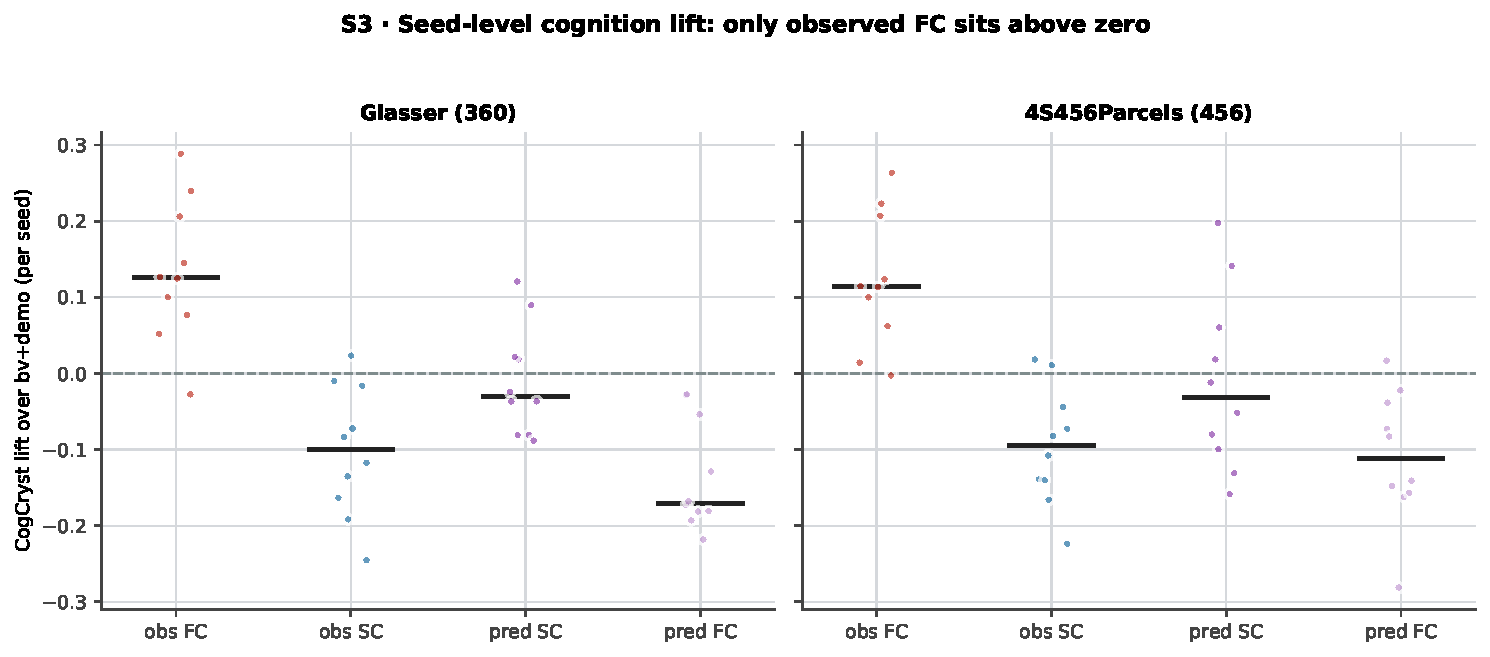
\includegraphics[width=0.88\linewidth]{S3_downstream_lifts.pdf}
  \caption{\textbf{Supplementary: seed-level cognition lift.} Per-seed lift over \bvdemo{} for CogCryst; only observed FC sits above zero.}
  \label{fig:s3}
\end{figure}

\FloatBarrier
\section{The Ceiling Is Structural in This Regime}

The negative downstream result could have several mundane explanations. The grid and supplementary checks test these explicitly (Figure~\ref{fig:escape}).

First, the cross-modal asymmetry is not an artifact of PCA reduction. In a reduction-axis sanity check, the \fcsc{} / \scfc{} ratio remained greater than 1.0 across learned PCA, full PLS on raw 64{,}620-edge vectors, and three Johnson--Lindenstrauss random projections. Median ratios ranged from $1.39\times$ to $1.81\times$ across methods, with Wilcoxon $p \le 0.001$ against a ratio of 1.0 for all methods.

Second, the ceiling is not recovered by richer models. KernelRidge and other nonlinear checks did not reveal hidden signal beyond the linear baselines; the KernelRidge $3\times3$ hyperparameter sweep was nearly degenerate, with within-seed spreads around $0.004$--$0.005$ in \dpear.

Third, richer structural representations did not help. Named-bundle tractography features predicted FC worse than streamline-count SC, added no marginal value over count-SC, and did not improve cognition above the subject-information floor.

Fourth, the \scfc{} shortfall is not explained by FC measurement noise. FC was noisy at the single-edge level but reliable as a whole connectome: the between-session FC reliability ceiling in Glasser was \texttt{demeaned\_r}$=0.491$ with fingerprint \texttt{top1}$=0.933$. \scfc{} captured only about 17\% of that reproducible FC signal. Moreover, a subject's \scfc{} prediction quality was essentially uncorrelated with that subject's FC reliability ($r=0.01$), and filtering to high-reliability subjects raised the ceiling without improving \scfc{} prediction. The measured gap is therefore not an FC-side noise artifact.

These checks do not prove that SC can never predict cognition. They make a narrower and more useful claim: in healthy young adults, under cross-sectional normal-range cognition, the missing utility is not recovered by obvious changes in dimensionality reduction, model class, structural representation, or sample size within this regime.

\begin{figure}[h]
  \centering
  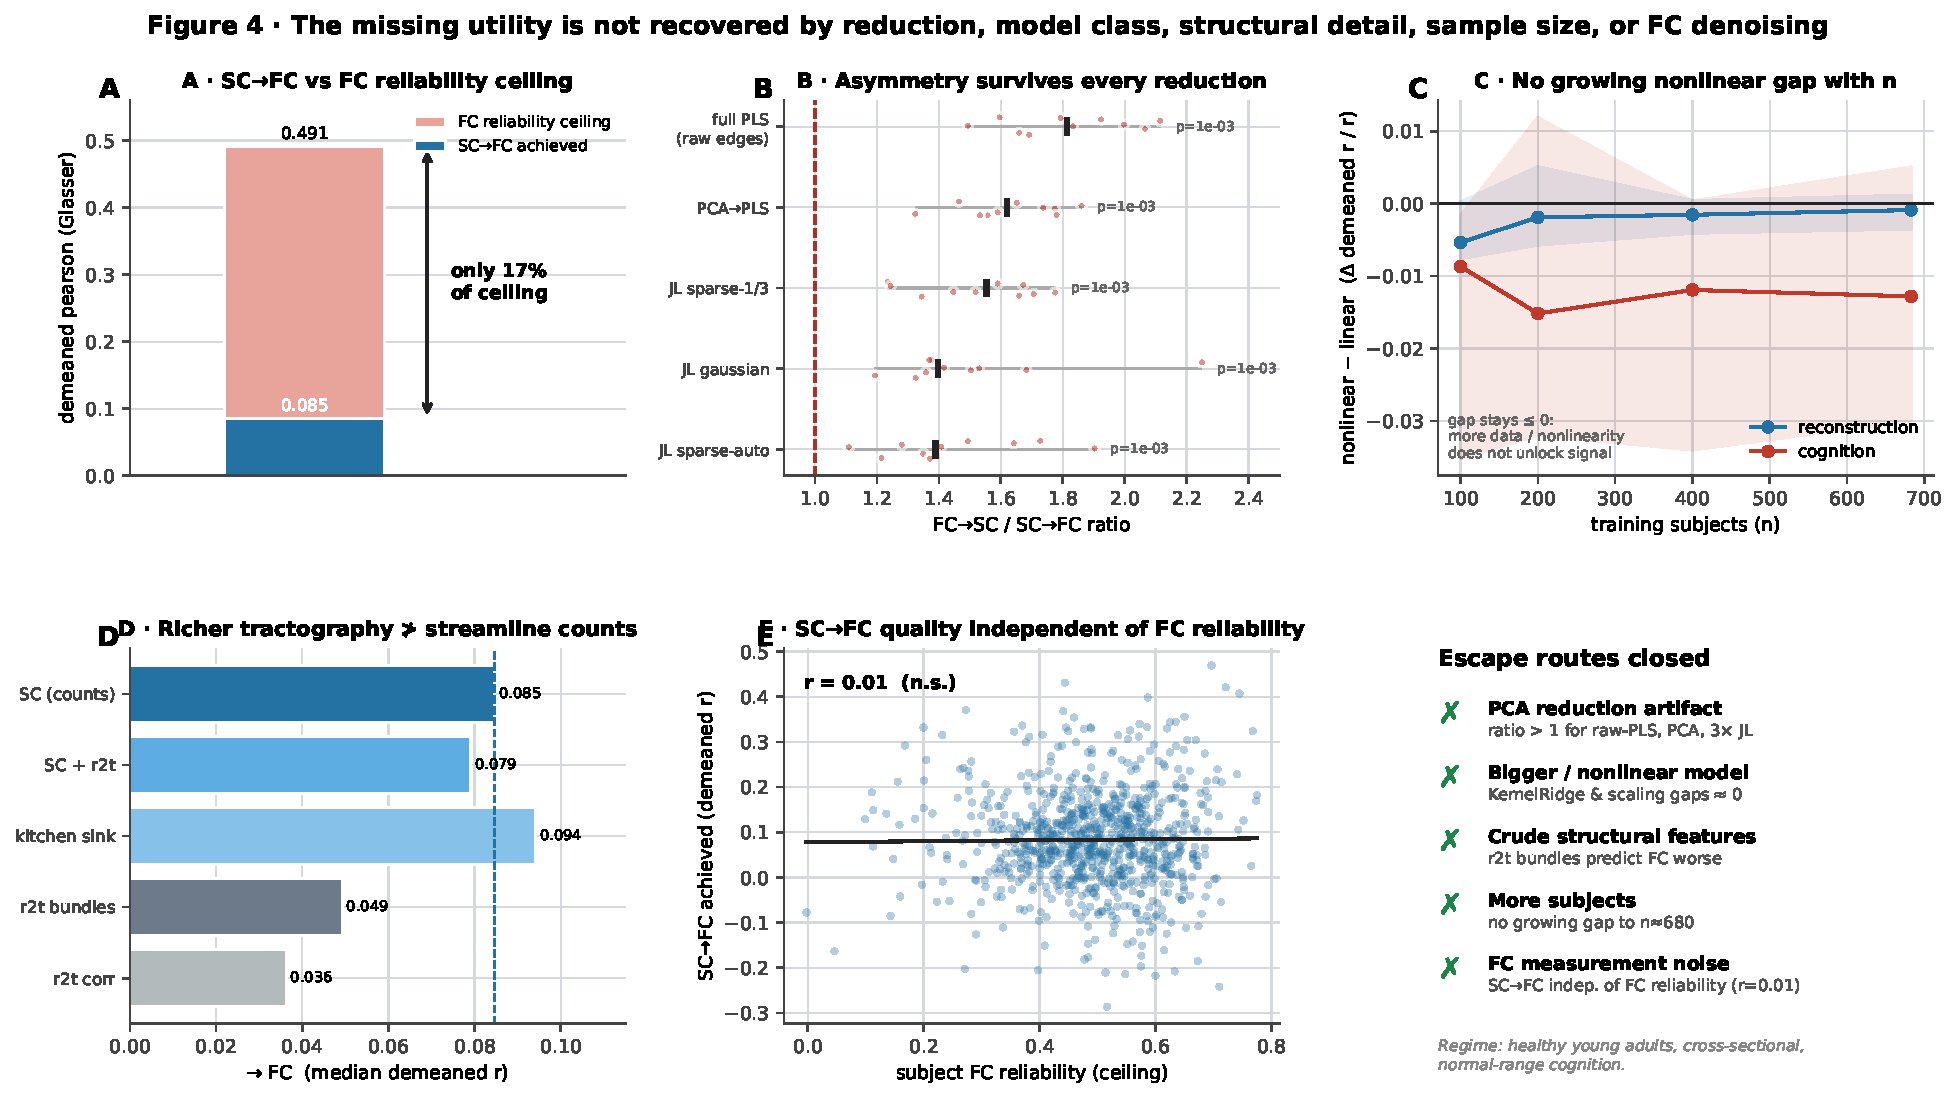
\includegraphics[width=\linewidth]{fig4_closed_escape_routes.pdf}
  \caption{\textbf{Closed escape routes.} (A) \scfc{} reaches only 17\% of the FC reliability ceiling; (B) the asymmetry survives every reduction axis; (C) the nonlinear-minus-linear gap does not grow with sample size; (D) richer tractography features do not beat streamline-count SC at predicting FC; (E) per-subject \scfc{} quality is independent of FC reliability; (F) summary of closed escape routes.}
  \label{fig:escape}
\end{figure}

\begin{figure}[h]
  \centering
  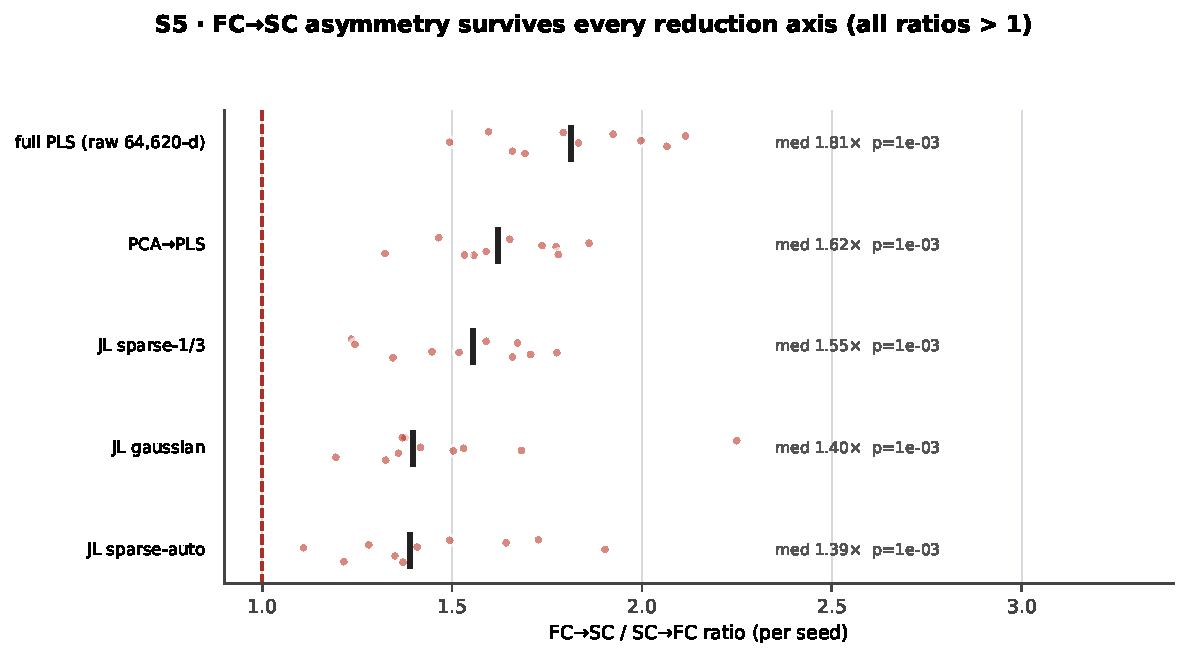
\includegraphics[width=0.8\linewidth]{S5_reduction_axis.pdf}
  \caption{\textbf{Supplementary: reduction-axis robustness.} The \fcsc{} asymmetry survives every reduction axis; all per-seed ratios exceed 1.}
  \label{fig:s5}
\end{figure}

\begin{figure}[h]
  \centering
  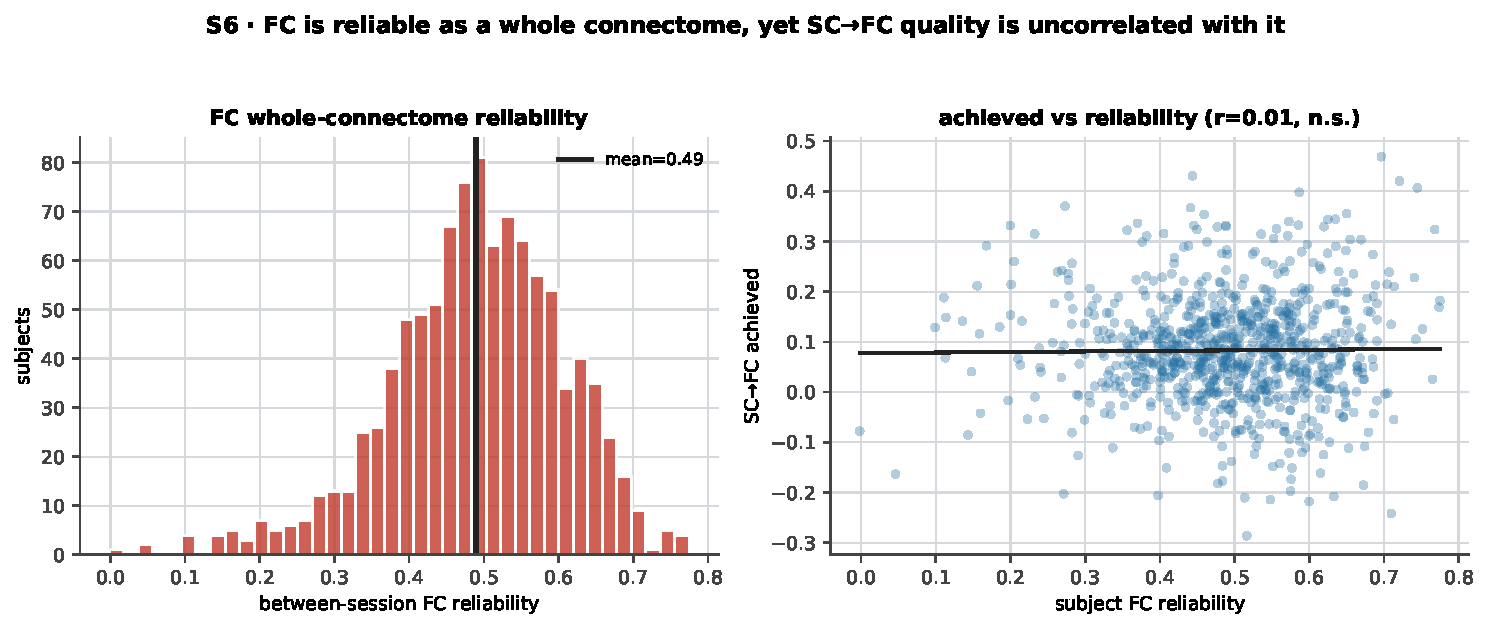
\includegraphics[width=0.88\linewidth]{S6_fc_reliability.pdf}
  \caption{\textbf{Supplementary: FC reliability.} FC is reliable as a whole connectome, yet \scfc{} quality is uncorrelated with it.}
  \label{fig:s6}
\end{figure}

\begin{figure}[h]
  \centering
  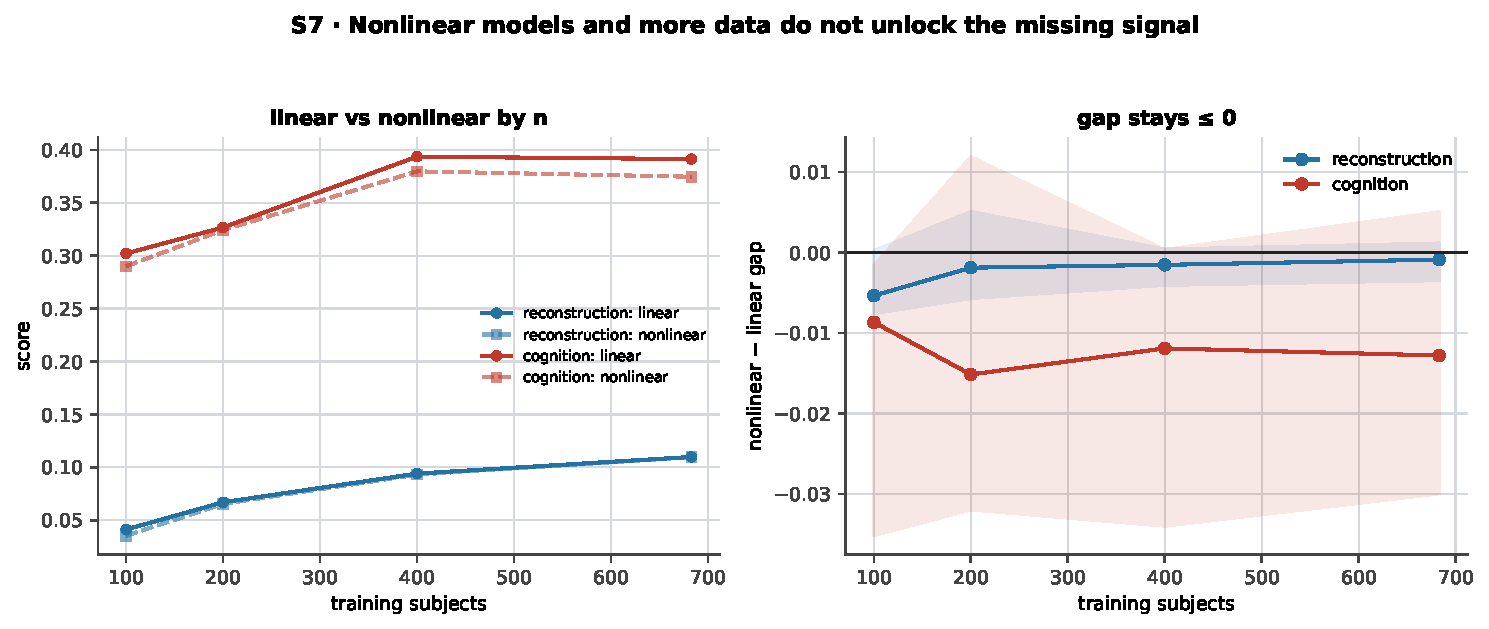
\includegraphics[width=0.88\linewidth]{S7_nonlinear_scaling.pdf}
  \caption{\textbf{Supplementary: nonlinear and scaling nulls.} Nonlinear models and more data do not unlock the missing signal.}
  \label{fig:s7}
\end{figure}

\begin{figure}[h]
  \centering
  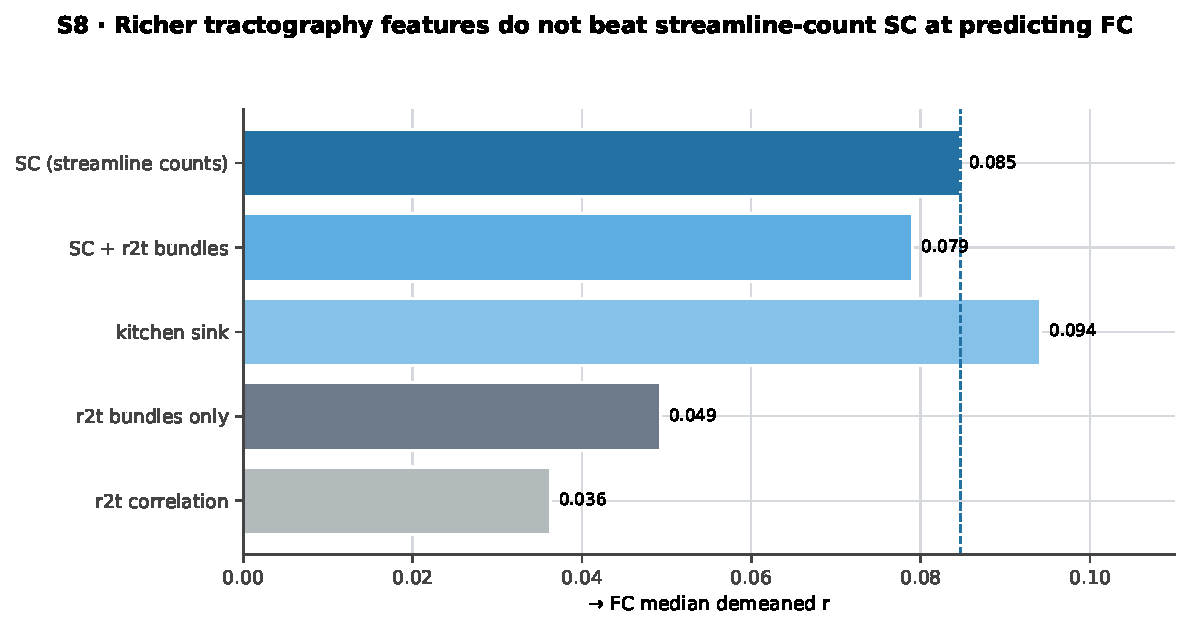
\includegraphics[width=0.72\linewidth]{S8_tractography.pdf}
  \caption{\textbf{Supplementary: richer structure.} Tractography (r2t) features do not beat streamline-count SC at predicting FC.}
  \label{fig:s8}
\end{figure}

\FloatBarrier
\section{Predicted Connectomes Carry Family Signal but Objectives Diverge}

The failure to improve cognition does not mean predicted connectomes are empty. Predicted SC from FC carried family structure. In both parcellations, \texttt{pred\_SC\_resid\_bvdemo} separated siblings from unrelated subjects with AUC around 0.81, far above the \bvdemo{} baseline around 0.56. This shows that cross-modal prediction can preserve individualized, heritable signal not reducible to the subject-information baseline.

However, the signal depends on the objective. A combined predictor optimized for reconstruction collapsed to chance for sibling separation, around 0.50 AUC, even though it performed well under reconstruction-style objectives. The practical lesson is that one predicted connectome cannot be assumed to serve every purpose. Reconstruction, cognition, and identification select different components of the data.

An exploratory mechanism analysis localized part of the family signal to a small, FC-predictable, low-variance SC mode. The exact component index was parcellation-dependent: the mode aligned with PC3 in Glasser and PC4 in 4S456Parcels. PC1 was dominated by sex and brain-volume confounding and should not be over-interpreted as biological mechanism. Because the mechanism effect is small and component labels migrate across atlases, we treat it as hypothesis-generating. The robust claim is the objective tradeoff, not a settled named-component mechanism.

\begin{figure}[h]
  \centering
  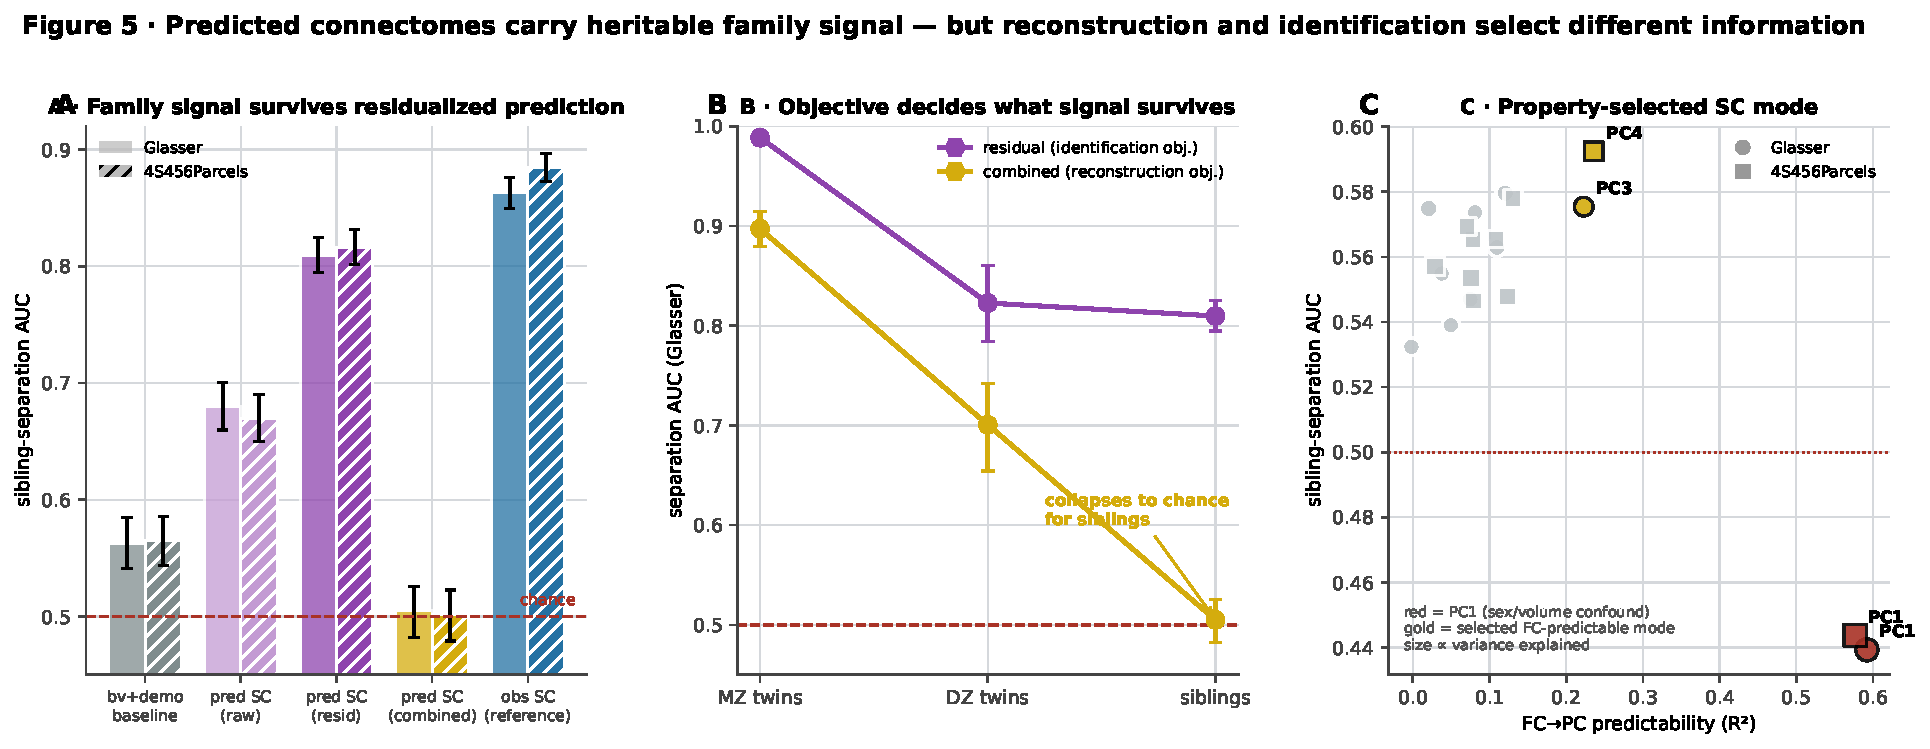
\includegraphics[width=\linewidth]{fig5_objective_divergence.pdf}
  \caption{\textbf{Signal changes with objective.} (A) sibling-separation AUC for baseline, raw, residualized, and combined predicted SC; (B) the reconstruction-optimized combined predictor keeps MZ/DZ signal but collapses to chance for siblings; (C) a property-selected FC-predictable low-variance SC mode (PC3 Glasser / PC4 4S456) carries the family signal, whereas PC1 is a sex/volume confound.}
  \label{fig:objective}
\end{figure}

\begin{figure}[h]
  \centering
  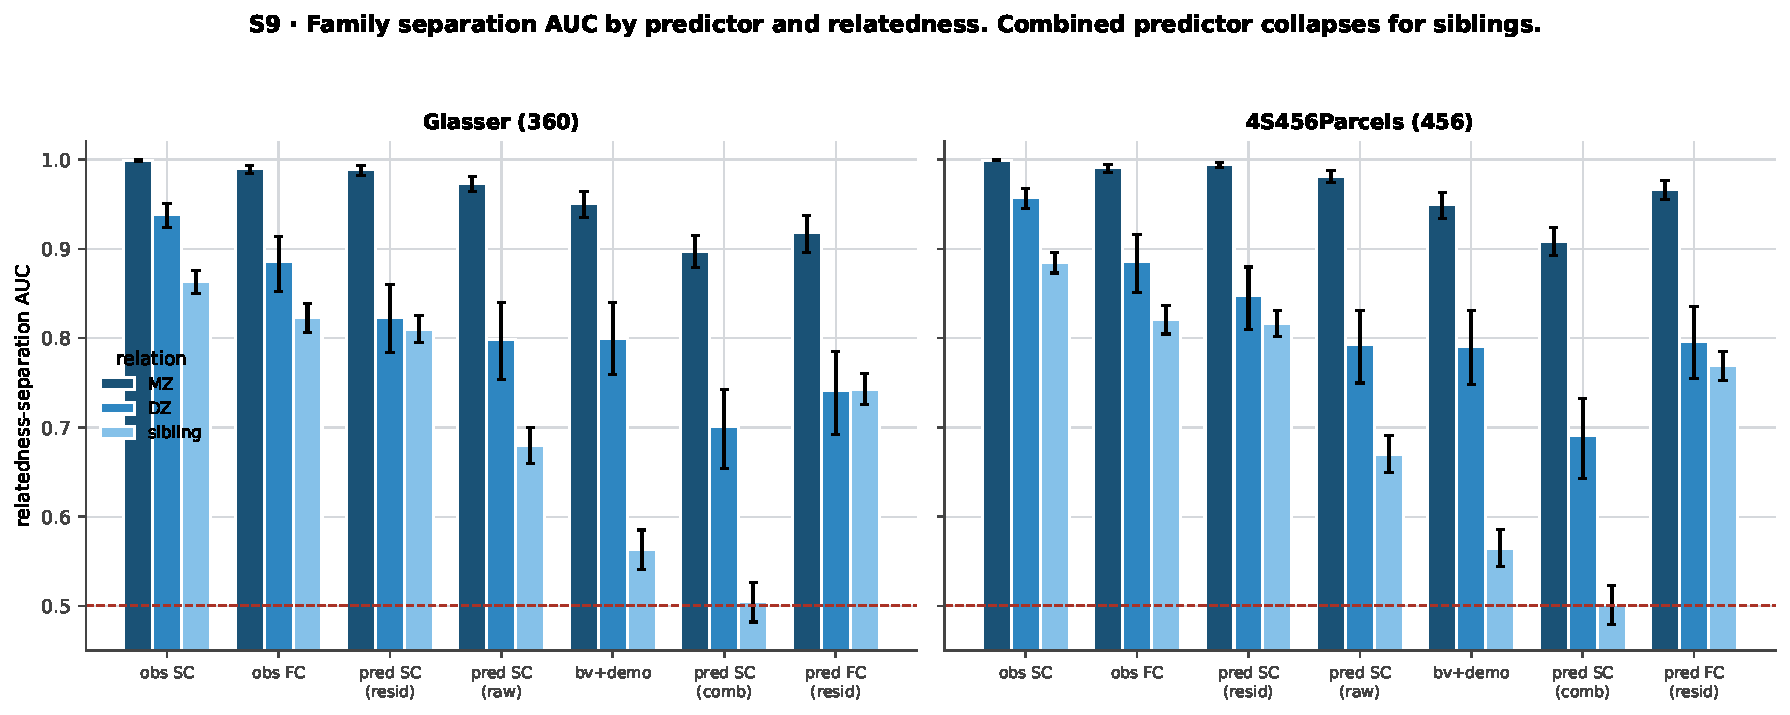
\includegraphics[width=\linewidth]{S9_family_auc.pdf}
  \caption{\textbf{Supplementary: family AUC.} Separation AUC by predictor and relatedness (MZ/DZ/sibling). The combined predictor collapses for siblings.}
  \label{fig:s9}
\end{figure}

\begin{figure}[h]
  \centering
  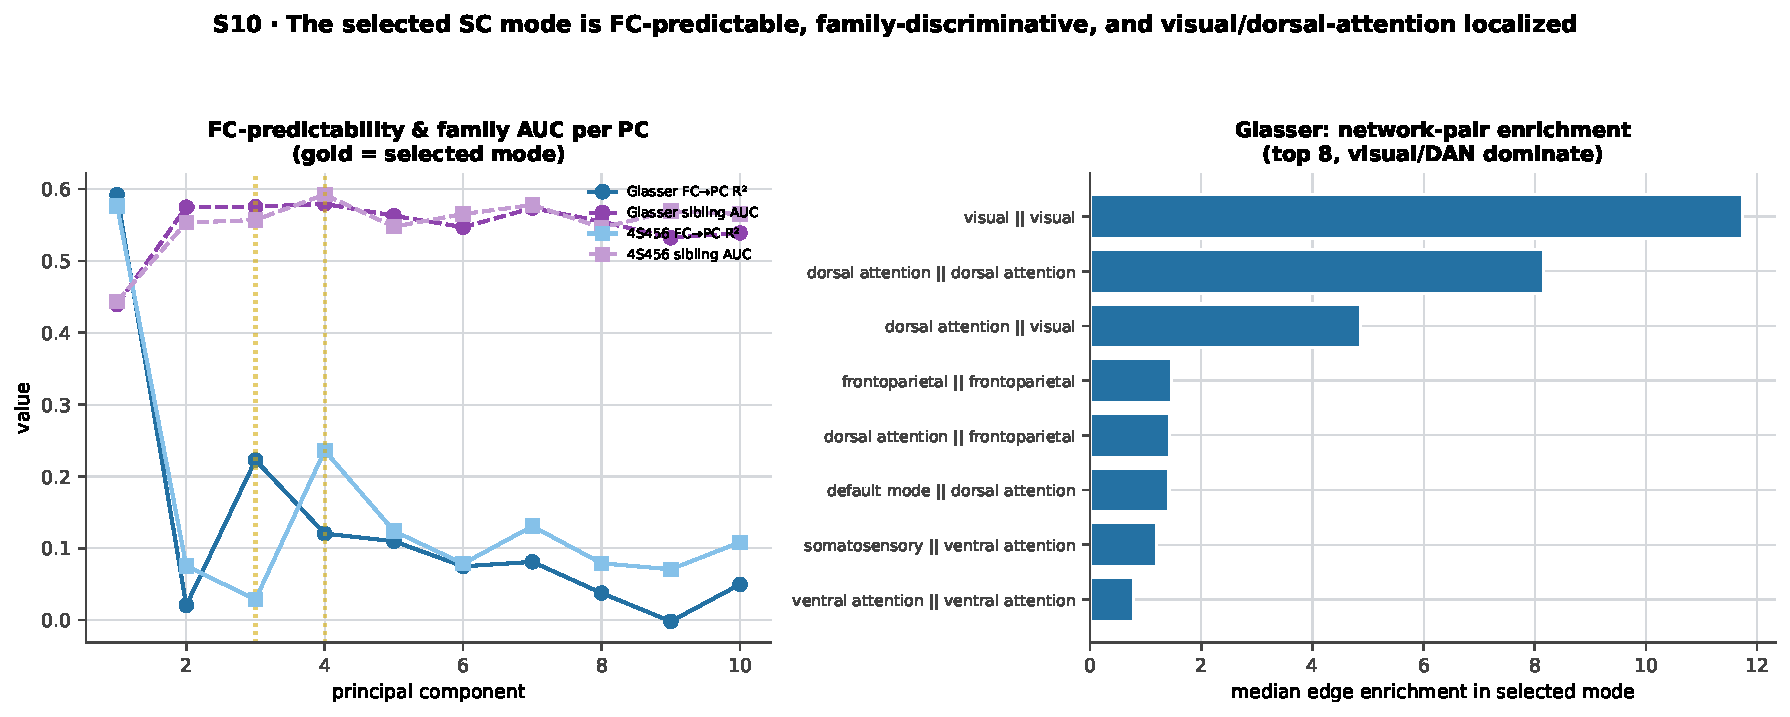
\includegraphics[width=\linewidth]{S10_pc_mechanism.pdf}
  \caption{\textbf{Supplementary: mechanism mode.} The selected SC mode is FC-predictable, family-discriminative, and visual/dorsal-attention localized.}
  \label{fig:s10}
\end{figure}

\FloatBarrier
\section{Discussion}

Cross-modal connectome prediction works, but it does not mean what it is often taken to mean. FC predicts SC better than SC predicts FC, and this directional structure is stable across atlases, seeds, and reduction checks. Yet downstream cognition tells a stricter story: observed FC helps, SC does not clear a cheap subject-information baseline, and imputed connectomes do not transfer utility from one modality to the other.

The main reporting implication is simple. Connectome translation papers should report:
\begin{enumerate}
\item Individual-deviation reconstruction metrics such as \dpear, not only raw population-mean-dominated correlations.
\item Same-modality oracle references, so cross-modal performance is placed against a model-capacity ceiling.
\item A cheap subject-information baseline such as \bvdemo{} for downstream behavior or cognition.
\item Separate evaluations for reconstruction, downstream prediction, and identification.
\item Split manifests, leak checks, and completeness checks for any large grid.
\end{enumerate}

The study also narrows where structural signal might still matter. The wall shown here is regime-specific: healthy young adults, cross-sectional data, and normal-range cognition. Clinical or lesioned populations, longitudinal designs, developmental change, or very large cohorts could expose structural signals that are weak or confounded here. The point is not to stop asking those questions. It is to carry the right checkpoint into them: does the connectome beat subject-level information?

\section{Limitations}

This is a single-cohort study in HCP Young Adults. The sample is healthy, young, and not representative of clinical or lifespan variation. The outcomes are normal-range cognitive measures, not diagnostic endpoints. SC test-retest data were not available in HCP-YA, so FC-side reliability could be measured directly but SC-side reliability remains data-blocked. The mechanism analysis is exploratory: the property replicates better than the component label, and its effect size is small. Finally, the negative results apply to this regime and these data; they should be treated as a strong checkpoint rather than a universal impossibility theorem.

\section{Conclusion}

FC--SC translation is reproducible, directional, and scientifically informative. But reconstruction accuracy alone is not enough. In HCP-YA, observed FC is the useful cognitive modality, SC and imputed connectomes do not beat cheap subject information for cognition, and predicted connectomes carry family signal only under objectives that preserve it. The field should therefore treat cross-modal prediction as a set of separable claims: reconstructability, downstream utility, and identity signal. Each needs its own baseline.

\end{document}
